\chapter{Comment réduire l'impact énergétique des data centers ?}
\vspace{3cm}
\minitoc
\clearpage
\label{Chapitre2}
\section{Introduction}
\begin{onehalfspace}
%L'idée est de concentrer les traitements de données sur une machine et d'éteindre les autres. Il est ainsi possible d'éteindre des supports stockant des archives « mortes » etc. Les constructeurs proposent des solutions en ce sens (support pour les archives plus lent à réagir mais consommant moins d'énergie).\medskip \\
%Il s'agit d'une piste d'économie d'énergie qui ne nécessiterait que peu de modification physique dans un data center et qui mérite une attention particulière.\medskip \\
%La première question qu'il faut donc se poser est comment réduire la consommation d'énergie. Différents moyens sont à notre disposition, certains étant au niveau du fonctionnement de la machine elle même, et donc à une granularité de phases d'application, alors que d'autres sont à des niveaux plus hauts, et donc à une granularité d'application entière. Certains sont basés sur des leviers matériels, alors que d'autres sont purement applicatifs.\medskip \\
%Il est pourtant possible de gérer les serveurs et les opérations informatiques que doit effectuer un data center pour monter le taux d'utilisation à plus de 95\% [5].\medskip \\
%\lettrine[nindent=1em,lines=3]{A}fin d'agir sur la consommation d'énergie des data centers, nous possédons un ensemble de moyens bien différents. Ces moyens sont à différentes échelles, mais chacun a un impact sur cette consommation, et des effets souvent négatifs sur les performances. Ainsi, nous avons des leviers qui vont d'un niveau bas, au niveau processeur ou au niveau machine, à un plus haut niveau, de cluster ou d'infrastructure. Ces leviers peuvent être aussi bien logiciels, comme la virtualisation, que matériels, comme le DVFS.
%\subparagraph{}Nous essayerons dans cette partie de présenter les mécanismes actuellement disponibles et les principaux travaux de recherches qui ont été proposés.


\lettrine[nindent=1em,lines=3]{C}omme tout autre système distribué, les datas centers des clouds font face à une demande croissante en énergie. Cette énergie ne provoque pas seulement la diminution des bénéfices des fournisseurs mais aussi émette une grande quantité de dioxyde de carbone. Afin d’agir sur cette  consommation, les travaux de recherches dans la littérature présentent un  ensemble de techniques  bien différents pour résoudre ce problème. Ces moyens sont à différentes échelles mais chacun a un impact sur cette consommation et des effets souvent négatifs sur les performances du système. Ces techniques sont appliquées soit  à un niveau bas comme le processeur, soit à un niveau plus élevé de cluster ou d’infrastructure au niveau machine. Ces techniques peuvent être aussi bien logiciels comme la virtualisation que  matériels comme le DVFS (voir la section \ref{DVFS}).\medskip
\subparagraph{}Nous allons présenter dans ce chapitre quelques différentes techniques d’optimisations d’énergie et les principaux travaux de recherches qui ont été proposés dans la littérature.

\end{onehalfspace}
\section{Dynamic Voltage and Frequency Scaling}
\label{DVFS}
\begin{onehalfspace}
Le DVFS est un mécanisme mis en place par les constructeurs de puces. Il permet de réduire ou d’augmenter dynamiquement la fréquence d’un composant ainsi que son voltage. Cela permet de diminuer la fréquence d’un processeur lorsqu’il est sous utilisé, ou au contraire, d’augmenter sa fréquence au dessus de sa fréquence maximale  lorsqu’il a besoin d’être plus performant. Ce mécanisme se fait en réglant un couple de voltage/fréquence (appelés "Performance state" PState) dont les valeurs dépendront du processeur utilisé.\medskip

Les différents couples voltage/fréquence sont gérés par le système de la machine. C’est le cas dans les systèmes où sont implémentés des gestionnaires de fréquence CPU qu'on appelle gouverneur. Le but de ces gouverneurs  est de gérer la fréquence et le voltage du processeur en fonction d’une orientation définie par l’utilisateur et en fonction de certains paramètres systèmes. Trois gouverneurs différents sont implémentés par défaut : \textbf{performance}, \textbf{powersave} et \textbf{ondemand}. Le gouverneur \textbf{performance} réglera la fréquence au maximum, le \textbf{powersave} règlera la fréquence au minimum. Le gouverneur \textbf{ondemand} quand à lui règlera la fréquence au maximum dès l’arrivée des tâches à effectuer, il réduit  petit à petit cette fréquence quand la charge baisse.\medskip 

Néanmoins, toute action a un coût et le DVFS n’y échappe pas et peut ralentir une  application. Changer la fréquence prend du temps (de l’ordre de dizaine de microsecondes \cite{ref10}). Ce temps passe sans calcul. Par conséquent, des changements courants de fréquence vont avoir un impact très négatif sur les performances du système. Cet impact induira évidemment à un mauvais temps d’exécution de l’application (si cette application termine), ce qui donne une mauvaise consommation d’énergie. Il est important de noter qu’un autre inconvénient de la technique DVFS existe. Il peut arriver qu’une application consomme plus en tournant à une fréquence plus basse. Prenons par exemple une application qui se termine en 10 secondes avec un processeur qui consomme 100 W à une fréquence maximale. Nous aurons donc une consommation d’énergie de 1000 Joules. Admettons maintenant que cette même application consomme une fréquence minimale  de 50W mais prend  un temps de calcul de 30 secondes. Nous aurons alors une consommation d’énergie de l’application de 1500 Joules. Par contre, si cette application se termine en 15 secondes à fréquence minimale, nous aurons une consommation de 750 Joules.\medskip 

%Pour palier au problème de l'augmentation de la consommation d'énergie à basses fréquences, dans [43] les auteurs définissent un ordonnanceur visant à allouer les tâches HPC sous contrainte d'un budget d'énergie à ne pas dépasser. Ils utilisent les capacités apportées par le DVFS pour régler la fréquence des processeurs en fonction de l'échéance et du ralentissement prédits des tâches. Les résultats observé par simulation sur plus de 4000 processeurs montrent que les algorithmes que les auteurs ont défini apportent une augmentation de performance allant de 20\% à 40\% pour les tâches en comparaison avec une approche sans DVFS, tout en respectant la borne sur la consommation d'énergie.\medskip \\
Une vitesse d'exécution réduite n'implique pas forcément une réduction de la consommation d'énergie. Ce qui signifie que la réduction de la puissance n'implique pas non plus une réduction de la consommation d'énergie. Un bon exemple est décrit dans \cite{ref11}, où les auteurs présentent et implémentent un algorithme de scheduling basé sur des événements pour le gouverneur de processeur. Pour ce faire, les auteurs ont implémenté un scheduler qui reçoit des événements en fonction de la charge de travail. Ainsi, si la charge était basse au dessus d'un certain seuil, l'événement "chargé" va être envoyé et le gouverneur va ainsi changer la fréquence du processeur.\medskip 

La comparaison est faite notamment avec les gouverneurs implémentés dans les noyaux  Linux qui sont : performance (avec une fréquence maximale) et powersave (avec une  fréquence minimale). On remarque dans les résultats présentés par les auteurs que le gouverneur performance exécute le programme en 1h03 avec une puissance de 310W, cela  résulte une énergie de 329 Wh. On remarque aussi que le gouverneur powersave exécute ce même programme en 3h09 à une puissance de 284W résultant une énergie de 895Wh.  L’algorithme proposé dans cet article  exécute ce même programme en 1h05 avec une puissance moyenne de 298W avec  une énergie de 324Wh. Cela montre bien qu’il est nécessaire de bien utiliser  la gestion de fréquence des processeurs. Une fréquence plus faible n’économisera pas forcément de l’énergie et le bon choix sera parfois de favoriser la performance pour économiser l’énergie consommée avec un temps d’exécution plus court.\medskip 


Les auteurs dans \cite{ref12} tentent de résoudre  le  problème d’affectation de la fréquence la plus efficace en énergie en utilisant la charge de travail par intervalle. Cela est fait pour allouer la bonne fréquence et le bon voltage aux tâches. Ils ont proposé  un gouverneur visant à réduire la consommation d’énergie en minimisant les pertes de performance, acceptant ainsi des pertes pour avoir une  meilleure économie d’énergie. Pour cela, les auteurs caractérisent la charge de travail pour chaque nœud. Ils définissent ensuite le gouverneur efficace en énergie ecod basé sur les moments où le CPU attend le résultat d’activités hors processeur. Cela caractérise la charge en se basant sur des mesures sans avoir besoin d’aucune connaissance des applications qui s’exécutent sur le cluster. L’algorithme est ensuite évalué par l’exécution des benchmarks NAS Parallel Benchmark \cite{ref13}. Les auteurs montrent qu’une économie d’énergie allant jusqu’à 11\% peut être effectuée par rapport au gouverneur \textbf{ondemand} avec une faible perte de performance (5.1\% d’augmentation du temps de calcul contre 7.9\% pour \textbf{ondemand}).\medskip 


Un autre inconvénient de taille pour le DVFS est l'impact de la fréquence du DVFS sur le fonctionnement du processeur. En effet, des études montrent que l'utilisation du DVFS a un impact négatif sur la fiabilité du processeur \cite{ref14}. Les auteurs montrent analytiquement que réduire la fréquence à voltage fixe tend à réduire la performance (c'est-à-dire la probabilité de finir une application correctement avant échéance lorsqu'il y a des erreurs). De plus, réduire le voltage à des fréquences réduites augmente le taux d'erreurs dans les processeurs. \medskip 

L'approche de type DVFS n'est pas seulement limitée aux processeurs. C'est une approche qui peut être appliquée aussi à d'autres types de matériels. Par exemple, nous pouvons utiliser une approche similaire au niveau des cartes réseaux. Celle-ci s'appelle l'Adaptative Link Rate (ALR) \cite{ref15}. Le principe est le même : augmenter ou baisser la vitesse de la carte (son débit, faire fonctionner une carte Ethernet 1Gbps à 100Mbps ou moins) en fonction des besoins afin de limiter la consommation d'énergie. %Nous pouvons aussi effectuer le contrôle du voltage et de la fréquence au niveau des GPUs (Graphics Processing Unit), puisque ceux-ci sont utilisés dans certaines architectures hybrides CPU/GPU, où certains calculs sont effectués sur le GPU d'une machine, alors que les autres sont fait sur le CPU. Les GPUs sont de plus traditionnellement plus performants en terme de performance par watts pour les tâches très parallélisables, en en faisant des matériels intéressants pour améliorer l'efficacité énergétique des serveurs comme montré dans \cite{ref16}. Les auteurs dans \cite{ref16} montrent de plus qu'identifier les moments où il faut changer la fréquence et le voltage dans une architecture hybride CPU/GPU, permet d'atteindre des économies d'énergie de 28\% avec seulement une baisse de 1\% en performance dans le cas d'additions et de multiplications de matrices.\medskip 

%Ce genre d'approche est de plus en plus utilisée. Nous verrons de plus en plus de composants avec différentes vitesses possibles, et nous utiliserons de moins en moins explicitement ces capacités, car les fonctionnements seront directement intégrés, soit au niveau matériel, soit au niveau du système d'exploitation. Le but étant de s'approcher le plus possible d'infrastructures matérielles dites "proportionnelles", c'est-à-dire qui ne consomment qu'une énergie proportionnelle à leur charge.
\end{onehalfspace}

\section{Allumage et extinction des machines}
\begin{onehalfspace}

Il existe un moyen simple pour réduire la consommation d'énergie d’une machine. Il suffit de l’éteindre !
Par éteindre, nous entendons une extinction totale de la machine pour amener sa consommation à 0W. Cela est  possible par des appareils permettant de "désactiver" les prises de courant \cite{ref33}. Il faut bien faire la distinction entre une extinction et une mise en hibernation. Ce sont deux états similaires mais qui ne consomment pas la même puissance.
L’extinction de la machine désigne l’arrêt total de tous ses composants en réduisant la consommation de puissance à un niveau proche de 0W. Nous désignerons par  hibernation l’arrêt du système à l’exception de certains composants utilisés pour la mise en veille du système. Comme exemple d’hibernation, nous citons la carte réseau par l’utilisation du \textit{wake-on-lan} (technique consistant à réveiller une machine à distance par le réseau), le \textit{suspend-to-RAM} ou le \textit{suspend-to-Disk}.

La Figure \ref{EmachineLinux} est un exemple de diagramme des différents états d’une machine Linux. Elle présente les coûts en temps et en puissance électrique nécessaire pour passer d’un état à un autre. Les valeurs présentées sont tirées de \cite{ref17}.\medskip
\clearpage
\begin{figure}[!htb]
\begin{center}
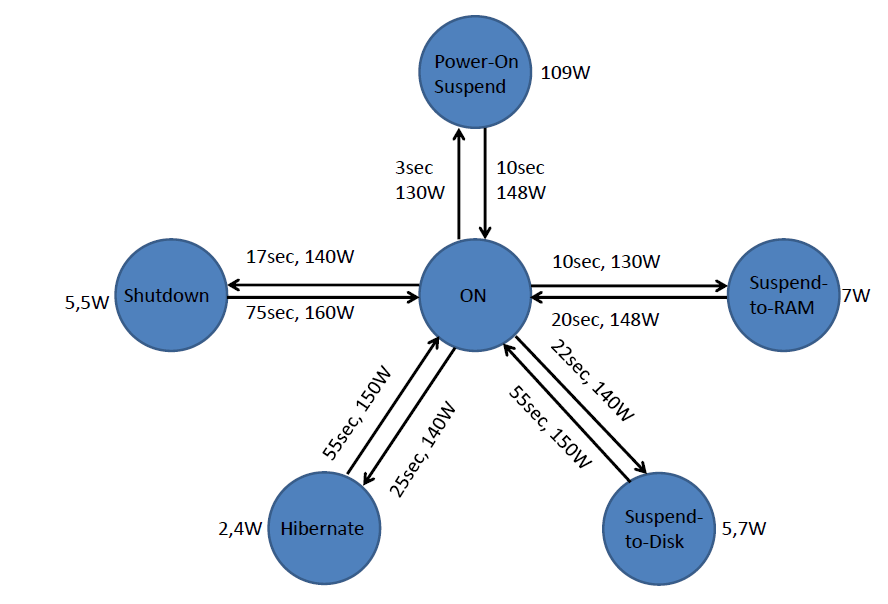
\includegraphics[scale=0.45]{figures/3.png} 
\end{center}
\caption{Exemple de transition entre états pour une machine Linux}
\label{EmachineLinux}
\end{figure}

Ainsi, il est possible de développer des approches utilisant cette technique afin de réduire
la consommation d'énergie. Dans \cite{ref18}, une approche utilisant un processus de décision de Markov est utilisée. Cette approche permet de  gérer les tâches,  l’état des hôtes (allumé ou éteint) et elle permet aussi d’atteindre l’état optimal pour la consommation d’énergie  tout en préservant la qualité de service (temps d’attente des tâches).\medskip

Cependant, pour réduire la consommation énergétique d'un serveur à 0W, nous devons prendre
en compte plusieurs facteurs.\medskip

Premièrement, nous devons être capables d’éteindre et de rallumer à distance les machines. Mais dans les clusters actuels, nous n’avons pas tout le temps cette capacité car les machines ne sont pas faites pour être éteintes. Deuxièmement, nous devons prendre en compte le temps pris pour éteindre et rallumer les différentes machines. Ce temps est équivalent au  temps pendant lequel les machines ne soient pas utilisées et consommeront de l’énergie. Il faut donc bien prendre en compte le temps d’allumage pour ne pas en avoir besoin en temps réel. Cela induit à une dégradation dans la qualité de service de la tâche. Enfin, il faut prendre en compte le coût induit par la consommation des ressources lors de l’allumage et l’extinction. C’est le cas lorsqu'on allume une machine. En plus du démarrage normal du système d’exploitation, cette machine  effectue une série de tests matériels et logiciels. Cela prend donc du temps mais aussi coûte de l’énergie dans la mesure où la machine fait des calcule. Ces temps et consommations d’énergie varient bien sûr en fonction de la machine, du système et des vérifications matérielles qui doivent être faites. Pour le temps d’allumage, cela peut aller jusqu’à la vingtaine de secondes dans \cite{ref19} à un peu plus d’une minute comme dans \cite{ref17}, voire même de plusieurs dizaines de minutes comme dans \cite{ref20}. \medskip


Toutefois, un effet indésirable peut apparaître lorsqu'on sollicite trop l'allumage et
l'extinction de matériels. Cela peut causer une augmentation du taux de malfonctionnement de
la machine. Bien que rien n'indique qu'au niveau machine le taux de malfonctionnement des hôtes ait
un lien avec le nombre de démarrage/extinction \cite{ref20}. Ce lien peut exister de la même manière  que pour le processeur et le DVFS comme c'est vu dans la section précédente \cite{ref14}.\medskip

L'allumage et l'extinction des hôtes physiques est donc une technique importante et extrêmement
puissante quand il s’agit de la réduction de  la consommation d’énergie d’un système informatique.
Ce moyen est  à utiliser avec précaution dans la mesure ou une mauvaise prédiction peut
causer des allumages/extinctions très fréquents  impliquant ainsi un gaspillage de ressources
et d’électricité. Il faut toujours que l'énergie économisée pendant qu'une machine reste éteinte soit plus
importante que celle consommée pendant l'allumage et l'extinction. C'est à dire augmenter la consommation d'énergie tout en dégradant la qualité de service.
\end{onehalfspace}

\section{Allocation}
\begin{onehalfspace}
L'allocation des tâches est aussi un moyen pour gérer la consommation d'énergie d'un système.
En plaçant de façon intelligente les tâches, nous pouvons utiliser les infrastructures les
moins gourmandes en électricité.\medskip

C’est le cas des techniques dites de consolidation. Le but étant de regrouper la charge de travail au même endroit pour pouvoir réduire la consommation d’énergie. Consolider les tâches sur un nombre réduit de machines peut avoir de graves effets. Outre le fait qu’on puisse tenter de consolider sans succès, il faut aussi prendre en compte les interactions que peuvent avoir les tâches entre elles lorsqu’elles s’exécutent sur une même machine. Dans \cite{ref21}, les auteurs montrent qu’en présentant la consommation de ressources d’une tâche, la consommation de ressources et l’énergie consommée par chaque transaction augmentent comparativement lorsqu’elle est seule. De plus, l’efficacité énergétique d’une transaction tend à augmenter aussi si la tâche s’exécute toute seule sur la machine. Les auteurs montrent ensuite qu’on peut trouver une zone optimale à laquelle chaque tâche s’exécutant sur la machine consommera le moins d’énergie. Ils proposent ensuite un algorithme de consolidation basé sur le profil des interactions des tâches pour déterminer la consolidation optimale ou proche de l’optimale, ainsi que pour caractériser quels types de charges de travail doivent être combinées.\medskip

L’allocation peut aussi être utilisée en tant que technique dans la mesure où une bonne caractérisation des différentes ressources matérielles peut faire une différence importante. Tous les serveurs ne consomment pas la même puissance pour exécuter la même application et donc l’utilisation de l’allocation des tâches s’avère donc importante. Différentes techniques peuvent être observées pour prendre en compte les différentes consommations à différents niveau, que ce soit au niveau du processeur ou au niveau de la machine elle-même.\medskip

C’est le cas par exemple de Dupont et al. dans \cite{ref22}, où les auteurs utilisent l’allocation et la réallocation des machines virtuelles pour mettre en oeuvre un framework flexible et efficace en énergie (ensemble de composants logiciels). Pour ce faire, les auteurs se basent sur  la gestion des clusters par la  programmation par contraintes sur Entropy \cite{ref23} afin d’être flexible en exprimant les différents objectifs pour les algorithmes. Cela donne la possibilité d’ajouter ou d’enlever des contraintes pour exprimer les contraintes SLA sans changer les algorithmes. Les auteurs valident ensuite leur framework par simulation et expérimentations. Ils montrent que dans un environnement cloud de test, leur approche permet de réduire jusqu’à 18\% d’émissions CO$_{2}$.

\end{onehalfspace}

\section{Virtualisation}
\begin{onehalfspace}
Au fur et à mesure que les systèmes deviennent de plus en plus complexes et les architectures de plus en plus diverses, il faut rendre transparent certains services. Il devient ainsi nécessaire d’avoir un accès commun à des ressources différentes pour faciliter le développement. C'est ici qu'intervient ce qu'on appelle la technique de  virtualisation. Cette technique permet de  rendre l’accès identique à plusieurs architectures. Par exemple, on peut avoir un accès virtualisé à des processeurs différents quel que soit leur constructeur ou leur méthode d’accès. La virtualisation peut être appliquée à plusieurs niveaux. Nous pouvons avoir la virtualisation du stockage où l'accès aux ressources de stockage sera transparent quel que soit l’endroit où se trouvent effectivement les disques durs et quel que soit  leur type (type normal, SSD, mémoire flash...) \cite{ref24}.\medskip 

Nous avons aussi  la virtualisation des machines virtuelles (VMs). Cela consiste à donner un accès complet à une infrastructure virtuelle qui apparait à l'utilisateur comme une machine complète (voir Figure \ref{Diagramme virtualisation avec un hyperviseur }). Cette technologie sert à donner à deux clients différents un accès chacun à une machine complète sur une même machine physique (PM). Cela permet d'avoir une meilleure sécurité dans le sens où même si on donne un accès administrateur à un utilisateur sur une machine virtuelle, ce dernier  ne pourra pas compromettre l'intégrité physique de la machine hébergeant la machine virtuelle \cite{ref25}. \medskip 
\clearpage
\begin{figure}[!h]
\begin{center}
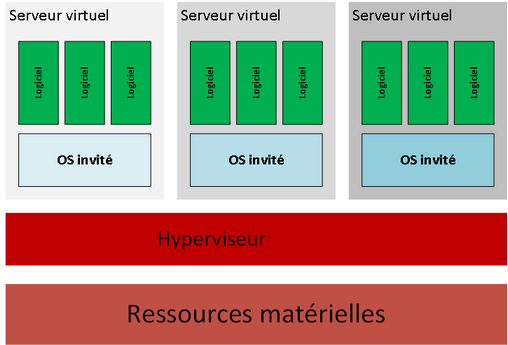
\includegraphics[scale=1]{figures/2.png} 
\end{center}
\caption{Diagramme virtualisation avec un hyperviseur }
\label{Diagramme virtualisation avec un hyperviseur }
\end{figure}


Les économies d'énergie réalisables grâce à la virtualisation sont de l'ordre de plus de 70\% à 80\%. Les économies réelles prélevées des projets de virtualisation dépendent du degré de virtualisation ainsi que du niveau de déploiement des nouvelles applications et fonctionnalités\cite{WEB26}.\medskip 

Les machines virtuelles ont l'avantage de permettre une séparation logique des ressources de la machine. Par exemple, on peut allouer deux machines virtuelles sur une même hôte en allouant par exemple 70\% du CPU à la première machine virtuelle et les 30\% restant à l'autre. Il apparaît donc que la gestion des tâches est facilitée par les technologies de virtualisation, notamment au niveau du pro-visionnement des tâches. Dans \cite{ref27}, les auteurs utilisent le fait que les machines virtuelles ne consomment pas tout ce qui leur est attribué pour sur-provisionner les machines physiques. Cela pour maximiser leur utilisation effective et économiser 20\% de ressources.\medskip 

La technique de virtualisation possède quelques inconvénients. Elle cause une baisse de performances. La gestion transparente des ressources est gérée par un intergiciel qui engendre des coûts de calculs et de gestion des ressources. Ainsi, un des inconvénients majeurs de la virtualisation est le surcoût associé à la virtualisation \cite{ref28}. Le surcoût est notamment dû au fait que d’une part l'accès aux ressources matérielles (GPU, disques durs, etc) est plus lent que l'intergiciel de virtualisation. Cet intergiciel  doit faire le lien entre le système hôte et la machine physique. Il est aussi dû au fait que les défauts de la page mémoire sont significativement plus coûteux. Ce surcoût dépend d'un certain nombre de paramètres tels que : le programme et l'architecture matérielle qui est virtualisée. Et peut atteindre des valeurs de ralentissement lorsque le cache est trop petit  (17\% pour une architecture Intel et 38\% pour une architecture AMD) \cite{ref28}.


\subparagraph{}La virtualisation offre une fonctionnalité nommée migration qui permet de migrer des machines virtuelles d'un nœud physique à un autre. Le but de cette technique est d'améliorer le temps de réponse et mieux gérer la consommation d'énergie.
\end{onehalfspace}

\section{Migration des machines virtuelles}
\begin{onehalfspace}
Les technologies actuelles de virtualisation permettent de migrer une machine virtuelle d'une machine physique à une autre. Cela peut se faire de deux manières. La première est une méthode qui consiste à mettre en pause la machine, la migrer et la reprendre une fois la migration terminée. La deuxième manière permet une migration dite à chaud. Il est possible de migrer une machine virtuelle presque sans perturber son fonctionnement, c'est-à-dire sans arrêter son fonctionnement mais avec une interruption de service minimale. Elle peut aller de 60ms pour un serveur de jeu à faible latence à 210ms pour un serveur avec un workload de type SPECweb99 \cite{WEB29}. Ce type de migration permet d'avoir une continuité du service avec juste une perturbation minimale au niveau réseau lors de la dernière partie de la migration \cite{ref30}.\medskip

Il existe plusieurs implémentations de la migration "live" de machines virtuelles. L'approche traditionnelle qui est implémentée dans Xen ou KVM par exemple est dite en pré-copie. Le processus de migration commence par une phase de pré-copie de la mémoire de
travail d'une machine virtuelle, puis va itérativement transférer à nouveau les pages qui ont
été utilisées par la machine virtuelle pendant le transfert précédent. Ceci jusqu'à l'obtention d'un
noyau de pages mémoire suffisamment petit ou jusqu'à ce qu'un nombre prédéfini d'itération
ait été effectué. La machine virtuelle est ensuite arrêtée et le noyau de mémoire final restant
à transférer est envoyé à la machine virtuelle destination qui est démarrée à son tour
marquant la fin de la migration.\medskip

Enfin, cette migration possède un coût non négligeable, qui entraîne une consommation de ressources sur l'hôte source et destination à la fois, ce qui augmentera la consommation d'énergie pendant la migration. De plus, les dernières phases de copie de la mémoire lors de la migration, juste avant de terminer celle-ci peuvent entraîner sur certaines machines une dégradation de la qualité de service. Par exemple, dans \cite{ref31}, les auteurs étudient le coût de la migration dans les clouds, avec des applications de type services web. Il apparaît que lors de la migration, le temps de réponse peut dans certains cas monter jusqu'à 3 secondes, induisant ainsi des violations de SLA\footnote{Le service level agreement (SLA) est un document qui définit la qualité de service requise entre un prestataire et un client.}.\medskip

Le coût de la migration peut être pris en compte dans la prise de décision afin de ne pas faire de ré-allocations de machines virtuelles et par conséquence ne pas perdre les  performances. C'est le cas de l'architecture de gestion de machines virtuelles de  GreenCloud proposé dans \cite{ref32}.

Il existe plusieurs techniques de migration des machines virtuelles, nous pouvons citer : la politique "Single Threshold" et la politique "Double Threshold".

\subsection{La politique "Single Threshold" (ST)}

La politique ST est basée sur l'idée de créer un seuil d'utilisation supérieur et de garder l'utilisation totale du CPU de toutes les machines physique en dessous de ce seuil.

\subsection{La politique "Double Threshold"}

L'idée est de fixer deux seuils, un seuil supérieur et un seuil inférieur et de garder l'utilisation totale du CPU de toutes les machines physiques entre ces seuils. L'objective de cette politique est de  réduire l'utilisation du processeur en dessous du seuil d'utilisation supérieur si le seuil supérieur est violé. Sinon si le seuil inférieur est violé, toutes les machines virtuelles doivent être migrées de cette machine physique et la machine physique doit être mise en état hors tension (etteinte). Nous allons définir maintenant les trois politiques basées sur la politique "Double Threshold".  

\subsubsection{La politique "Minimization of migrations" (MM)}

La politique MM sélectionne le nombre minimum de machines virtuelles nécessaires pour une migration.

\subsubsection{La politique "highest potential growth" (HPG)}

Lorsque le seuil supérieur est violée, HPG migre les machines virtuelles qui ont la plus faible utilisation de la CPU par rapport à la capacité de CPU définie par les paramètres des VMs. Cela pour minimiser l'augmentation potentielle de l'utilisation de l'hôte et et pour empêcher une violation SLA.

\subsubsection{La politique "The random choice" (RC)}

RC repose sur une sélection aléatoire d'un certain nombre de machines virtuelles nécessaire pour diminuer l'utilisation du processeur  en dessous d'un seuil d'utilisation supérieur.

\end{onehalfspace}
\clearpage
\section{Conclusion}
\begin{onehalfspace}
Dans ce chapitre, nous avons présenté quelques techniques d'optimisation d'énergie des data centers, en utilisant certains concepts tels que la virtualisation, la migration et la technique DVFS. Certaines techniques sont au niveau composant et d'autres sont au niveau infrastructure. Il convient donc de choisir les bonnes techniques pour arriver aux meilleurs résultats d'économies d'énergie et une bonne optimisation. Cela avec une perte minimale de performance et de qualité de service.

Le chapitre prochain consiste à implémenter une nouvelle stratégie de migration des machines virtuelles, Et cela dans le but d'améliorer certaines métriques de performance telle que la consommation d'énergie.
\end{onehalfspace}